% -----------------------------------------------
% Vlastní text práce (kapitoly práce)
% -----------------------------------------------

% -----------------------------------------------
\chapter{Gamma rays properties and matter interaction}
% -----------------------------------------------


% -----------------------------------------------
\section{Gamma emission}
In opposite to alpha and beta particles, the gamma rays are without charge and their rest mass is zero, and thus they are considered to be high-energetic photons, but the mayor difference to the X-Ray photons they originate only from atomic nucleus upon its deexcitation from higher energy level to lower. The energy levels of nucleus are similar to the levels in electron shell - discrete, characteristic for every isotope and can be described by quantum numbers. The gamma emission is usually follows alpha or beta decays. The gamma photon is emitted, because the new nucleus is created in an excited state.


% -----------------------------------------------
\section{Passage of radiation and particles through matter}
Interaction of a particle (radiation) with another particle (atom, nuclei, free electron) or with continuous matter can result into many types of reactions and effects - scattering of a particle from incident direction, creation of new particles and nuclei, annihilation of incident particle etc. It mainly depends on particle's energy, electric charge, spin and mass, but also on the properties of target particle or matter. The physical quantity describing the probability of a specific interaction of particle with single point target is known as the cross section. Normalized to the unit solid angle - differential cross section:



 \begin{equation}
\frac{d\sigma}{d\Omega} = \frac{1}{F} \frac{dN_\textrm{s}}{d\Omega}
 \end{equation}
Where $F$ is a particle flux, $\Omega$ is a solid angle and $N_\textrm{s}$ is the average number of scattered particles per unit time.
And the total cross section is given by integration:
  \begin{equation}
 \sigma = \int \frac{d\sigma}{d\Omega} d\Omega
 \end{equation}

However, to characterize the interaction probability of particle with continuous matter, which contains many interaction centres (defined by their density), other assumptions have to be made. The average number of scattered particles is given by:

 \begin{equation}
 N(\Omega) = FAN \delta x \frac{d\sigma}{d\Omega}
 \end{equation}


and integrated:

 \begin{equation}
 N_{tot} = FAN\sigma \delta x 
 \end{equation}

The $A$ is a total area perpendicular to the flux, $\delta x$ is the material thickness and $N$ is the density of interaction centres.
\par 
 
Heavy charged particles (such as alpha particles, protons, muons, pions) lose their energy mainly due to the atomic electrons collisions. Due to their mass which is much higher than the mass of electrons ($M >> m_\textrm{e}$) they collide with, the direction of their path is left unchanged. The loses of energy per unit path is defined as stopping power $\frac{dE}{dx}$. The stopping power for the heavy charged particles is given by Bethe-Bloch formula which relates stopping power and particle's energy. However the Bethe-Bloch formula doesn't apply on low energies (Lindhard-Sharf nuclear loses) and on higher energies (bremsstrahlung radiation). The change of their path direction is possible by the second process with lesser probability - by the elastic scattering from nuclei.
\par
Electrons and positrons have much smaller mass than the heavy charged particles, and thus the direction of their path is changed due to the movement in an electric field of nucleus. The bremsstrahlung radiation loses are mayor yet at low energies. However, the energy lost due to the collisions also comes to play - it is guided by special Bethe-Bloch formula, which takes the path direction change into account. 
\par

Other interaction effects are also possible (Cherenkov radiation emission, nuclear reactions), but they are rare or does not affect the particle's energy as those previously mentioned.

\par
The interaction of neutrons is totally different due to the lack of charge. 

\par

The interaction effects for gamma rays are described more detail in the following chapter.



\subsection{Gamma matter interaction}

Due to the fact, that the gamma rays are photons, the gradual losses of kinetic energy inside materials (characteristic for the charged particles) are not observed. Instead the main observed effect is the attenuation of intensity of photon flux with the increasing thickness of the absorber material. 

\par
Three mayor interaction effects of gamma photons and matter are Photoelectric effect, Compton scattering and Pair production. The cross section of these effect vary with gamma photon energy, with material and its density - high dependence on atomic number $Z$. There are also possible nuclear reaction such as the Mössbauer effect, but their observation requires very special conditions to be met.


\par
The attenuation of of photon flux has a form of exponential decay:

\begin{equation}
 I = I_{0}exp(-\mu x)
 \end{equation}
where $I_{0}$ and $I$ are the intensities and the parameter $\mu$ is the total absorption coefficient, which describes the probability of interaction per unit length and is bounded with total cross section of single atom $\sigma$ (combination of cross section of three main effects) by relation:

\begin{equation}
 \mu = N \sigma = \sigma(N_{a}\rho/A)
 \end{equation}
 
where $N$ - density of atoms, $N_{a}$ - Avogadro number, $\rho$ - material density and $A$ - molecular weight.

\par
The dependence of total cross section combined of the three main effect for lead on photon energy can be seen on fig. \ref{cross}.

\begin{figure}[H]
 \centering
 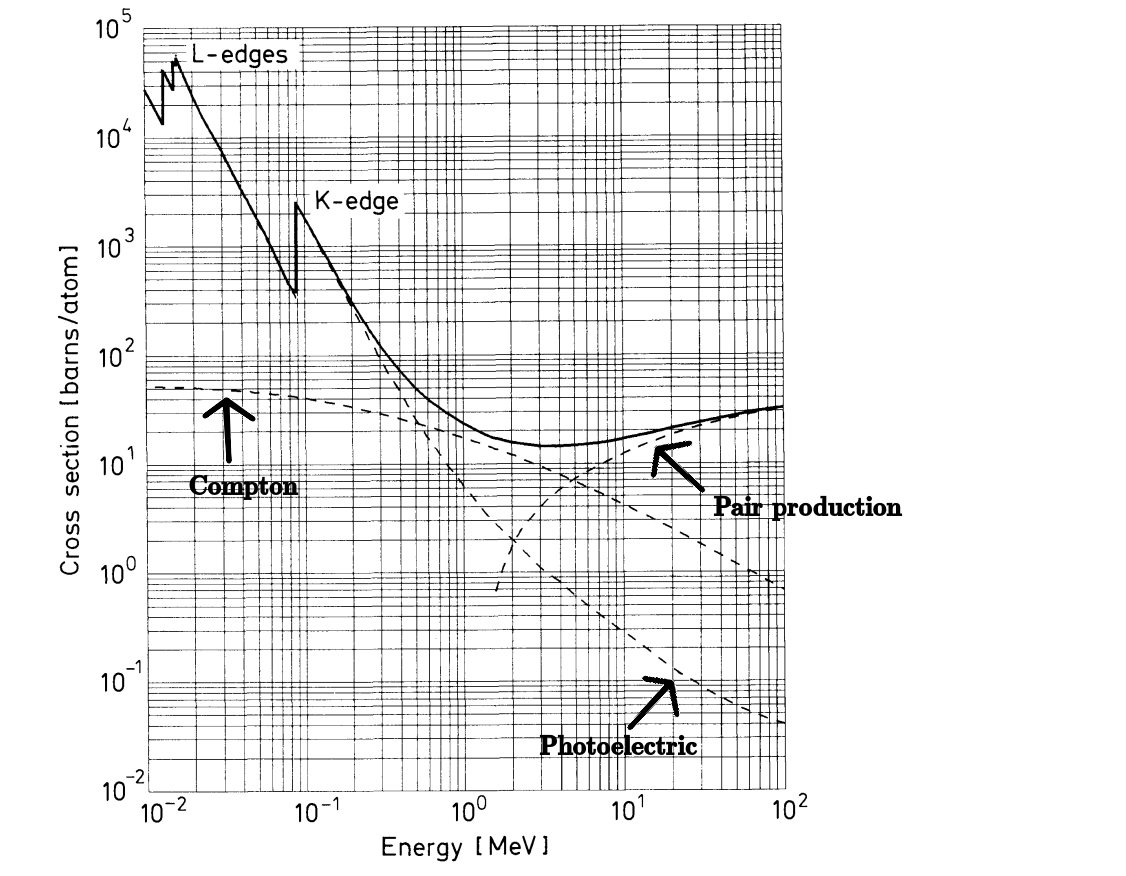
\includegraphics[scale=0.6, angle = 0]{./pictures/totalCross}
 \caption{Total absorption cross section for high-energy photons. Taken and modified from \cite{Leo1987-wy}.}
 \label{cross}
 
\end{figure}
 


\subsubsection{Photoelectric effect}
The photon is absorbed by electron from atomic shell. The electron is ejected and acquires the kinetic energy given by well-known equation:
 \begin{equation}
 E = hf - E_{b},
 \end{equation}
where $f$ is the photon frequency and $E_{b}$ is the binding energy.
 
The Photoelectric effect can be observed only on electron bounded in atomic shell, due to the fact, that the nuclei can absorb the photon's momentum. The cross section usually falls with energy and can have characteristic peaks from K,L,M transitions.

\par

The photoelectric effect plays the key role when it comes to the detection of gamma photons.

\subsubsection{Compton scattering}
Compton scattering is an effect, which is mainly observed on free electrons. It needs to be said, that the electrons in material are usually bounded, however, if the photon energy is much higher than the binding energy 
\par
This effect causes, that the photon loses only a part of its energy and changes its direction. The energy is transferred to an electron accordingly to the laws of energy and momentum conservation.

\subsubsection{Pair production}
At much higher energies, the photon can be converted into electron-positron pair. This effect happens near the nucleus, which absorbs a part of the original photon momentum.
\par
The pair production along with electron bremsstrahlung radiation  are key effects for electron-photon shower development. If the created electron/positron has sufficient energy, it emits bremsstrahlung photons. These bremsstrahlung photons can again interact via the pair production, and thus creating new electrons again. This process of shower development continues until the energy of electron/positron pairs drops under the energy, which is required to produce bremsstrahlung radiation.
\par
Negative effects arising from this type of interaction like creation of single and double escape peaks or annihilation peaks in spectra will not be observed, because for low-energy gammas the cross-section is very small. That means that for the purposes of this thesis, this interaction effect could be neglected.   


\subsection{Characteristic energy spectra}
Every gamma source emits its characteristic photons with certain probabilities. However, before these photons are captured by detector, many effects can occur in environment or inside the detector - photons can interact various materials without detection purpose such as shielding, spectrum can be altered by 
noise events in detector etc.
\par
Inside detector the low-energy spectre can be affected by:
\begin{itemize}
\item X-ray escape peaks - If the photo-effect occurs on atomic energy levels, the characteristic X-ray of the detector material is emitted. The escape peak has the energy of captured photon minus the energy of escaped gamma ray.
\item Compton continuum with edge - the photon interacts inside detector by Compton scattering, scattered photon leaves the detector.

\end{itemize}

In environment the low-energy spectre can be affected by:
\begin{itemize}
\item Characteristic X-rays - radiation induced fluoresce usually from the shielding material (Pb).
\item Backscatter peak - Compton scattering which occurred over a large angle.
\end{itemize}


For Mössbauer spectroscopy the $^{57}$Co is usually used with gamma spectre shown below:


% %%%%%%%%%%%%%%%%%%%%%%%% End of file %%%%%%%%%%%%%%%%%%%%%%%%